% This is samplepaper.tex, a sample chapter demonstrating the
% LLNCS macro package for Springer Computer Science proceedings;
% Version 2.20 of 2017/10/04
%
\documentclass[runningheads]{llncs}
%
\usepackage{graphicx}
% Used for displaying a sample figure. If possible, figure files should
% be included in EPS format.
%
% If you use the hyperref package, please uncomment the following line
% to display URLs in blue roman font according to Springer's eBook style:
% \renewcommand\UrlFont{\color{blue}\rmfamily}
\usepackage{amsmath}
\usepackage{multirow}
%\usepackage[margin=0.5in]{geometry}
       

% set the document title, author, and date here.
%  once set, the \maketitle command (within the document)
%  will display them nicely

\title{CS3243 Group 25 Project 2: Sudoku Solver}
\titlerunning{CS3243 Project 2: Sudoku Solver}
\author{Choong Jin Yao (A0173247A), Dominic Frank Quek (A0173261L),\\ Yang Shuqi (A0177383U), Yang Yiqing (A0161424N)}
\authorrunning{Choong J. Y., D. F. Quek, Yang S., Yang Y.}
\institute{National University of Singapore}

\begin{document}
\maketitle

\section{Problem Specification}
CSP search algorithm uses the structure of states and heuristics to solve problems. We are given the task of implementing a Sudoku solver using backtracking algorithm and heuristics. 

The puzzle is modeled as a list of 81 cells where each cell is represented by a (x, y) coordinate where $ 1\leq \verb`x,y` \leq 9$. Every cell is assigned a value \verb`v` where  $ 0\leq \verb`v` \leq 9$. An empty cell is where $v = 0$. The variables are the coordinates of empty cells in the given input puzzle. A list \verb`unassigned_var_list` contains the unassigned variables. The constraints are that for any of the 9 rows, 9 columns and 9 subgrids, no value can appear more than once. To enforce this constraint, at the start, we initialise 27 lists containing the legal values for each row, column and subgrid after removing the pre-assigned values in the given input puzzle. Then, we keep track of the domain of each variable containing its legal values. The domains are updated to be consistent with the 27 lists. 

Afterwards, we begin the backtracking algorithm. A state is represented by the \verb`unassigned_var_list` and \verb`assignments`. When a value is assigned to a variable, the variable is removed from \verb`unassigned_var_list`, its domain becomes empty and \verb`assignments` is updated. After every assignment, we use heuristics to remove illegal values from the domains of neighbouring variables. Hence, the constraints are guaranteed to be non-violated throughout.

An assignment is complete when the  \verb`unassigned_var_list` is empty. Afterwhich, we add the \verb`assignments` to the original puzzle.

\section{Algorithm variants}
We implemented a backtracking solver that incorporates heuristics in 3 aspects: Variable Ordering, Value Ordering and Inference

\subsection{Variable Ordering}
We prioritized the variable for expansion that is the most constrained.

\subsubsection{Most Constrained Variable: Minimum Remaining Value (MRV)} 

MRV chooses the variable with the least number of legal values, or equivalenty, smallest domain size.

\subsubsection{Most Constraining Variable: Degree}

Degree heuristic acts as a tie-breaker for the MRV heuristic. Among variables that have least and equal domain sizes, the variable with the most unassigned neighbours is prioritized.

\subsection{Value Ordering: Least Constraining Value}

Least Constraining Value heuristic prioritizes the value of a variable that results in the minimum reduction in the domains of neighbouring variables. In our implementation, we count the number of conflicts between the value and the values of its neighbours. A conflict happens when the value of the target variable is contained in the domain of its neighbour. The value with the least number of conflicts is prioritized. 

\subsection{Inference}

Inference is effective in reducing the domains of variables. Whenever a value is assigned to a variable, we can infer new domain reductions on its neighbouring variables. 

\subsubsection{Forward Checking}

Forward Checking ensures that a value assignment is consistent with the domains of all its neighbouring variables. Fundamentally, it ensures that the assigned variable is arc-consistent with the other variables. FC prunes the the domain values of variables that are in conflict with the value assignment. Failure is detected when any of the reduced domains is empty as a result.

\subsubsection{AC-3}

Whereas FC ensures arc consistency between a certain variable and the other variables, AC-3 ensures arc consistency between any 2 variables after every value assignment. This requires an initilisation of binary constraints where we create a tuple for each pair of neighbour variables. After every assignment, we loop through the binary constraints, reducing the domains whenever necessary. Whenever a domain is reduced using the \verb`revise` function, the binary constraints of the neighbours are added to the queue. Evidently, this can be computationally expensive. 

\section{Experimental Setup}

We run different variants of the aforementioned heuristics. Particularly, we tested the variant FC+AC3+MRV+LCV, where we used AC3 for post-processing for FC heuristic. 

We compare the perfomance of each variant by measuring the running time. This allows us to compare the efficiency of the variants in terms of time. The runtime of the variant accounts for all the work done and computations by the involved heuristics.

We find it inaccurate to compare the search space of different variants via computing the number of traversed nodes. It is impossible to establish a fair definition of what a node represents due to the different implementations of various heuristics. For instance, for AC-3, on top of the number of value assignments made before arriving at a solution, it also requires checking every binary constraint everytime an assignment occurs. For FC, it requires traversing the domains of remaining unassigned variables. One way to resolve is simply to define it to be the number of assignments made (equivalently, the number of calls to the \verb`recursive_backtrack` function. However, that is clearly too trivial as the additional work done by the heuristics is not accounted for. 

We also test the variants on the world's hardest Sudoku puzzle(Fig 1) found online (https://www.conceptispuzzles.com/index.aspx?uri=info/article/424).

\begin{figure}
\centering
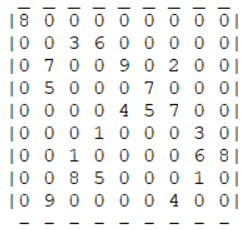
\includegraphics[scale=0.9]{hardest_sudoku.png}
\caption{World's Hardest Sudoku}
\label{Figure 1}
\end{figure}

\section{Results and Discussion}

The results for runtime performance are given in Fig 2 and 3. Runtimes longer than 300 seconds are indicated by a '-' symbol. 

Overall, AC3+MRV+LCV is the fastest, followed by FC+AC3+MRV+LCV, then FC+MRV+LCV. Hence, our implementation uses AC3+MRV+LCV.  

AC3+MRV+LCV turns out to be spectacularly much faster for hard puzzles(input1, hardest). Comparing it to FC+AC3+MRV+LCV, FC slows performance as it could be that failure detection by FC rarely occurs especially for hard puzzles, hence most of the extra work done is in vain as it still has to perform AC3. Comparing to FC+MRV+LCV, AC3+MRV+LCV is faster for all but 2 of the simpler puzzles(input2, 3). The explanation is similar to the one in the following paragraph.

Between FC+AC3+MRV+LCV and FC+MRV+LCV, FC+MRV+LCV is faster for easier puzzles, whereas FC+AC3+MRV+LCV is faster for harder puzzles. By inserting AC3 for additional post-processing, it leads to a chain reaction of domain reductions and thus detects failures faster than FC alone. Especially for hard puzzles, it enforces early termination and decreases the time for checking invalid assignments significantly. For simple puzzles, however, the reduction in runtime due to smaller search space in AC3 is outweighed by the reduction in runtime due to less computation in FC. After each assignment, AC3 has to ensure arc consistency between every 2 variables, whereas FC simply ensures consistency between a certain variable and other variables. This is further confirmed when you compare AC3 and FC in Fig 3.

Nonetheless, choosing the stronger but more computationally expensive AC3 is still preferred to FC because the time difference for simple puzzles is small($\leq 0.1s$), whereas for harder puzzles, the time difference becomes significant, up to 2 times faster (comparing AC3 and FC).

Implementing Degree heuristic, denoted by D, slows down the search. This is because the increase in time spent on computing the degree of every variable outweighs the reduction in time due to smaller search space. In fact, the purpose of the Degree heuristic is merely for tie-breaking for MRV. It is not worth the extra work of computing the degree. 

It can also be noted that MRV and LCV play a significant role in the decrease in runtime.   

\begin{figure}[ht]
    \begin{center}
        \begin{tabular}{ |c|c|c|c|c|c|c|c|c|  } 
        \hline
        Run time (seconds)        &FC+MRV+LCV+D   &AC3+MRV+LCV+D   &FC+MRV+LCV   &FC+AC3+MRV+LCV \\
        \hline
        \multirow{3}{0em}{} 
Sudoku (input1)             &0.912		         &0.826  			&0.347		 &0.251\\
        \hline
        \multirow{2}{0em}{} 
Sudoku (input2)             &0.082	          	 &0.085		        &0.003		 &0.016\\
        \hline
        \multirow{2}{0em}{} 
Sudoku (input3)             &0.009    		 &0.052		        &0.002		 &0.023\\

        \hline
        \multirow{2}{0em}{} 
Sudoku (input4)             &0.018     		 &0.012		        &0.019	  	 &0.004\\
        \hline
        \multirow{2}{0em}{} 
Sudoku (hardest)          &0.901			 &0.825	  		&0.349		 &0.253\\
        \hline
        \end{tabular}\\
        \caption{Experiments performed to measure runtime with various heuristics on Sunfire}
    \end{center}
\end{figure}

\begin{figure}[ht]
    \begin{center}
        \begin{tabular}{ |c|c|c|c|c|c|c|c|c|c|c|  } 
        \hline
        Run time (seconds)      &AC3+MRV+LCV &FC+MRV  &FC+LCV &AC3+MRV  &AC3+LCV	&AC3       &FC \\
        \hline
        \multirow{3}{0em}{} 
Sudoku (input1)             	 &0.020	       &0.912       &-		&0.616	 &-			&120.42   &236.654 \\
        \hline
        \multirow{2}{0em}{} 
Sudoku (input2)                  &0.013           &0.013	&0.095	&0.022	&0.033		&0.141     &0.520    \\
        \hline
        \multirow{2}{0em}{} 
Sudoku (input3)             	 &0.012	     &0.023	     &0.002		&0.146	&0.023		&0.023     &0.110    \\

        \hline
        \multirow{2}{0em}{} 
Sudoku (input4)             	 &0.011	    &0.011       &0.003		&0.802	&0.011		&0.018	&0.350   \\
        \hline
        \multirow{2}{0em}{} 
Sudoku (hardest)                &0.020         &0.926	      &-		&0.614	&-	       		&120.390  &236.671\\
        \hline
        \end{tabular}\\
        \caption{Experiments performed to measure runtime with various heuristics on Sunfire}
    \end{center}
\end{figure}












\end{document}
